\documentclass{article}
\title{EECS 345 Written 1}
\author{Patrick Landis (pal25)}

\usepackage{amsmath}
\usepackage[margin=1in]{geometry}
\usepackage{tikz}
\usepackage{tikz-qtree}

\begin{document}
\maketitle

\section*{Problem 1}
\begin{tabular}{l l c c c c c}
$<E>$ & $\rightarrow$ & $<V> = <E>$ & $|$ & $<COND>$ \\
$<COND>$ & $\rightarrow$ & $<OR> ? <E> : <E>$ & $|$ & $<OR>$ \\
$<OR>$ & $\rightarrow$ & $<OR> || <COND>$ & $|$ & $<AND>$ \\
$<AND>$ & $\rightarrow$ & $<AND> \&\& <NOT>$ & $|$ & $<NOT>$ \\
$<NOT>$ & $\rightarrow$ & $!<PAREN>$ & $|$ & $<PAREN>$ \\
$<PAREN>$ & $\rightarrow$ & $(<E>)$ & $|$ & $<V>$ & $|$ & $<BOOL>$\\
$<BOOL>$ & $\rightarrow$ & $TRUE$ & $|$ & $FALSE$ \\
$<V>$ & $\rightarrow$ & 1$|$2$|$3$|$4$|$5$|$6$|$7$|$8$|$9$|$0 \\
\end{tabular}

\section*{Problem 2}
\subsection*{Problem 2a}
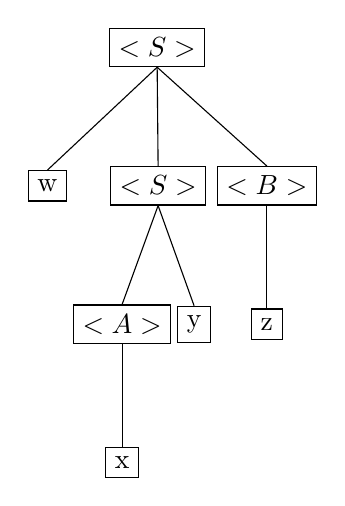
\begin{tikzpicture}[every tree node/.style=draw]
\tikzset{level distance=50pt}
\Tree [.$<S>$ w [.$<S>$ [.$<A>$ x ] y ] [.$<B>$ z ] ]
\end{tikzpicture}

\subsection*{Problem 2b}
Impossible there can't be a y before z in the parse tree. \\
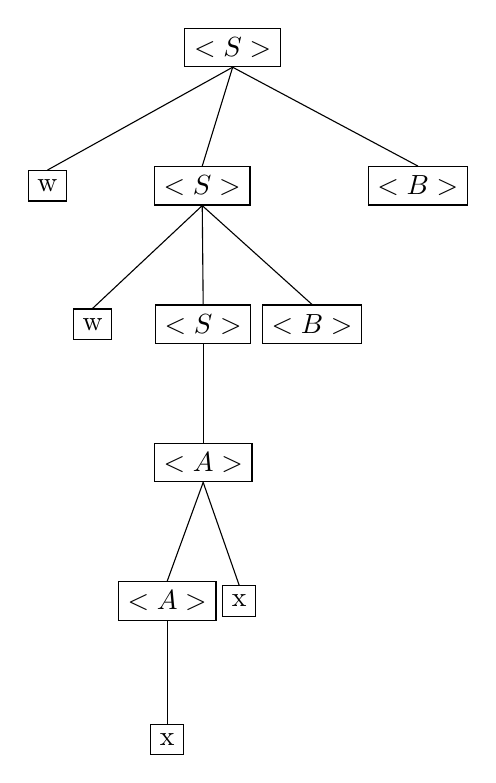
\begin{tikzpicture}[every tree node/.style=draw]
\tikzset{level distance=50pt}
\Tree [.$<S>$ w [.$<S>$ w [.$<S>$ [.$<A>$ [.$<A>$ x ] x ] ] $<B>$ ] $<B>$ ]
\end{tikzpicture}

\subsection*{Problem 2c}
Impossible, x+ (one of more x's) proves this cant be done. \\
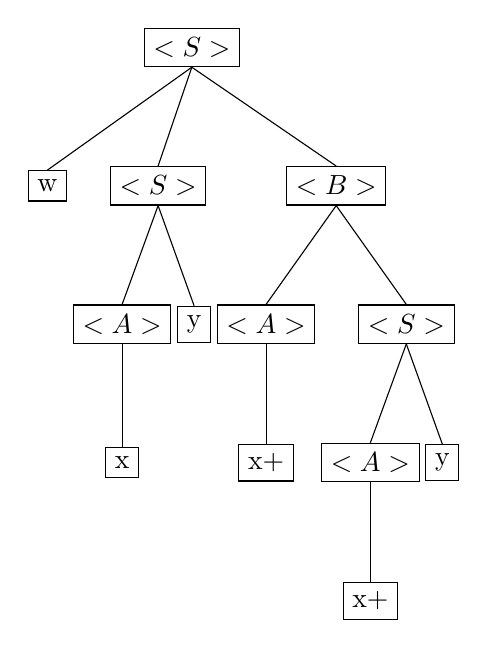
\begin{tikzpicture}[every tree node/.style=draw]
\tikzset{level distance=50pt}
\Tree [.$<S>$ w [.$<S>$ [.$<A>$ x ] y ] [.$<B>$ [.$<A>$ x+ ] [.$<S>$ [.$<A>$ x+ ] y ] ] ]
\end{tikzpicture}

\subsection*{Problem 2d}
Impossible, x+ (one of more x's) proves this cant be done. \\
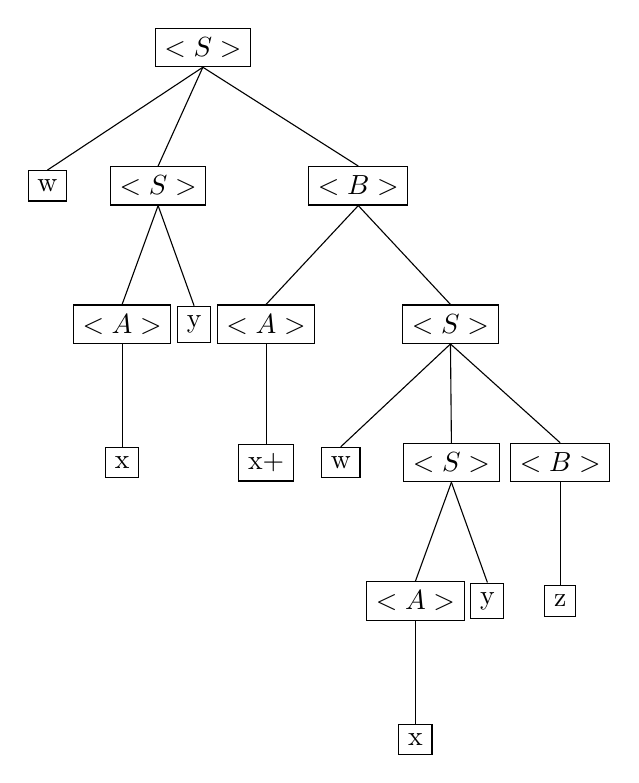
\begin{tikzpicture}[every tree node/.style=draw]
\tikzset{level distance=50pt}
\Tree [.$<S>$ w [.$<S>$ [.$<A>$ x ] y ] [.$<B>$ [.$<A>$ x+ ] [.$<S>$ w [.$<S>$ [.$<A>$ x ] y ] [.$<B>$ z ] ] ] ]
\end{tikzpicture}

\subsection*{Problem 2e}
Possible \\
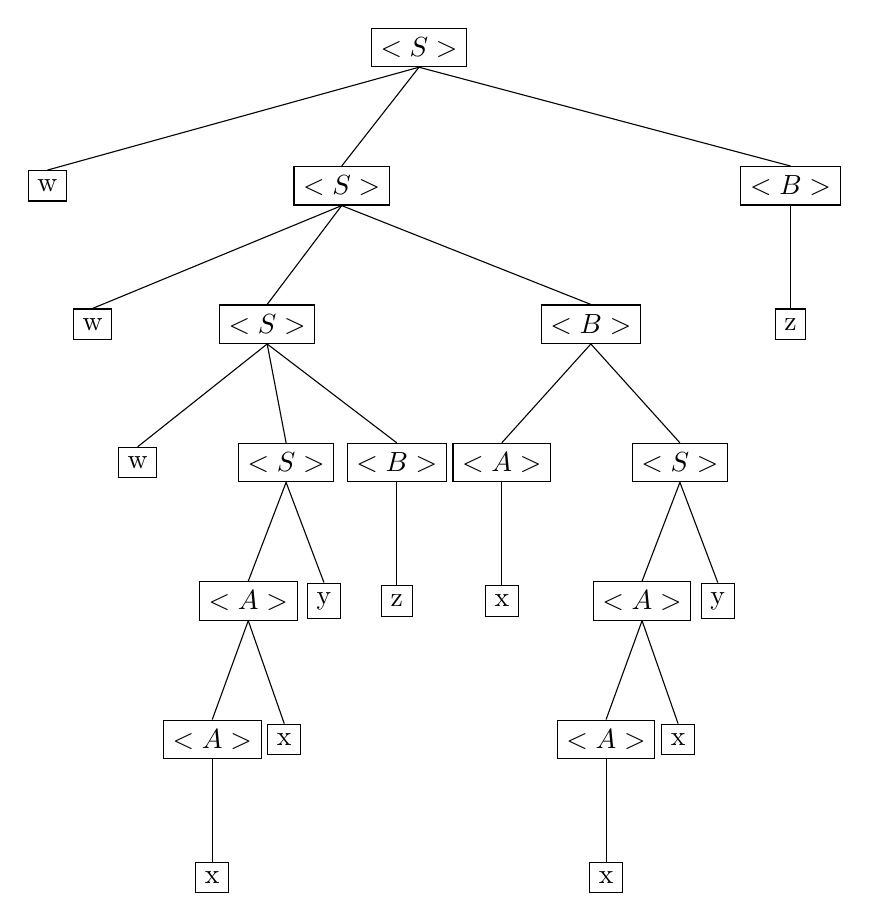
\begin{tikzpicture}[every tree node/.style=draw]
\tikzset{level distance=50pt}
\Tree [.$<S>$ w [.$<S>$ w [.$<S>$ w [.$<S>$ [.$<A>$ [.$<A>$ x ] x ] y ] [.$<B>$ z ] ] [.$<B>$ [.$<A>$ x ] [.$<S>$ [.$<A>$ [.$<A>$ x ] x ]y ] ] ] [.$<B>$ z ] ]
\end{tikzpicture}

\section*{Problem 3}
\subsection*{Problem 3a}
\begin{verbatim}
M_state(<var> = <expression>, s)
{
    if(M_value(<var>, s) != err)
        s = Remove(M_name(<var>, s)
    
    return Add(M_name(<var>), M_value(<expresion>, s), s)
}
\end{verbatim}

\subsection*{Problem 3b}
\begin{verbatim}
M_state(while <cond> <loopbody>, s)
{
    if(M_boolean(<cond>, s) == false
        return s
    else
       return M_state(while <cond> <loopbody>, M_state(<loopbody>, s))
}
\end{verbatim}

\section*{Problem 4}
\subsection*{Problem 4a}
\begin{tabular}{| l | c | r |}
\hline
Pre-Cond & Line & Post-Cond \\ \hline
$(y<0, x>2y)$ & & \\ \hline
(if $y<0$, then $x>2y$) & $y = y - x$ & ($x>-2y$) \\
(if $y\geq0$, then $x>0$) & & \\ \hline
$(x>-2y)$ & $x = x + 2 * y$ & $(x>0)$ \\ \hline
& & $(x > 0)$ \\ \hline
\end{tabular} \\ \\

Weakest because $2y < 0$

\subsection*{Problem 4b}
\begin{tabular}{| l | c | r |}
\hline
Pre-Cond & Line & Post-Cond \\ \hline
$(a*x \geq 2*b)$ & & \\ \hline
($a*a*x \geq 2*b$) & if($a>0$) then $y=a*a*x-b$ & ($y\geq b$) \\ \hline
($a*x \geq 2*b$) & else $y=a*x-b$ & $(y\geq b)$ \\ \hline
& & $(y\geq b)$ \\ \hline
\end{tabular} \\ \\
Weakest because a*a*x will always be greater than a*x

\subsection*{Problem 4c}
Pre-Condition: low$\leq$high, i$\geq$p, p$<$q \\ \\
Post-Condition: $A[p]<$low$\leq$high$<A[q]$ \\ \\
Since we know nothing about the section where this code is being used we know nothing about the ordering of the values in A. Instead we can reason about where in the array we are accessing.

\section*{Problem 5}
While-Loop LI: A[bound] $<=$ ... $<=$ A[n-1] \\ \\

Initialization: bound = n so there are no values in the array. \\
Maintainence: After each loop the bound-th largest element is bubbled to the sorted part of the array \\
Termination: bound is 0 which means that A[0] $<=$ A[1] $<=$ ... $<=$ A[n-1] and the post-condition is met. \\

\end{document}